\chapter{Revisión de la literatura}

En este capítulo se revisa el estado actual de la literatura relacionada con el problema, prestando especial atención a las dos vertientes sobre las que se basa el estudio: aquellas técnicas ya aplicadas para resolver el problema del EEG y el estado del arte actual en cuanto a algoritmos de optimización de miles de variables, con el objetivo de establecer el símil sobre el que se basa el desarrollo de este Trabajo de Fin de Grado. 

\section{Estado del arte: \textit{EEG Problem} y propuestas de solución}

En el año 2015, durante el IEEE Congress on Evolutionary Computation llevado a cabo en Sendai, Japón\cite{IEEE-CEC2015}, se presenta la  \textbf{Optimization of Big Data 2015 Competition}\cite{CompetitionBigOpt} donde, a diferencia de años anteriores, no se propone un conjunto de funciones benchmark de alta dimensionalidad sino un problema completamente distinto, el de la optimización de los datos de un electroencefalograma, que ha sido descrito en el capítulo anterior.

Si bien no se conocen con exactitud todas las técnicas propuestas para esta competición, cuando los organizadores publican su artículo \textit{Evolutionary Big Optimization (Big Opt) of Signals}\cite{EvolutionaryBigOpt}, en el que se recogen los resultados obtenidos al aplicar el problema sobre dos \textit{state-of-the-art} \textbf{MOEAs}, algoritmos evolutivos multiobjetivo: MOEA/D y NSGA-II.

\textbf{MOEA/D}\cite{MOEA/D} emplea la estrategia de descomposición para hacer frente a los problemas multiobjetivo: descompone el problema MO en un subconjunto de problemas y los optimiza de forma separada utilizando únicamente la información de los subproblemas vecinos, reduciendo considerablemente la complejidad del problema en cada generación si lo comparamos con el algoritmo \textbf{Nondominated Sorting GA II} (NSGA-II)\cite{NSGA-II}, que posee una complejidad de orden $O(MN^2)$ siendo \textit{M} la cantidad de objetivos y \textit{N} el tamaño de la población; el algoritmo crea una \textit{mating pool} donde la población de padres y offsprings se combinan, eligiendo posteriomente el mejor de estos, dando solución a los impedimentos típicos de los algoritmos MO que utilizan clasificación no-dominada.

En el artículo mencionado anteriormente, se propone el enfoque \textbf{multiobjetivo}, optimizando por separado ambas funciones \ref{eq:function1} y \ref{eq:function2}. Se elige optimizar dos representaciones distintas, frente al \textbf{dominio del tiempo} y frente al \textbf{dominio de la frecuencia}; este último para intentar superar los inconvenientes derivados de la dimensionalidad del problema.

Los resultados muestran un mejor desempeño de \textbf{MOEA/D} frente a NSGA-II en la representación frente al dominio de la frecuencia, dado que esta, a través de una \textbf{Fast Fourier Transform} aplicada sobre los componentes principales, es capaz de reducir \textbf{hasta la mitad la dimensionalidad} del problema (con una frecuencia de 1Hz). La r\textbf{educción de la dimensionalidad} y los\textbf{ buenos resultados} conseguidos son las principales bazas a tener en cuenta de cara a una aplicación real donde los datos de un EEG sean procesados y posteriormente ``blanqueados" por algoritmos evolutivos multiobjetivo.

\subsection{MAGA-BigOpt: Algoritmo Genético Multi-Agente para optimización uniobjetivo}

\textbf{MAGA-BigOpt}, \textit{A Multi-Agent Genetic Algorithm for Big Optimization Problems}\cite{MAGA-BigOpt}, es la principal propuesta de solución para el problema del EEG formulado en la Optimization of Big Data 2015 Competition, con enfoque uniobjetivo. Esta técnica, basada en un framework MAGA, ``r\textit{eestructura los operadores de competición y autoaprendizaje, que finalmente combina con operadores de cruce y mutación para \textbf{simular la cooperación, competición y comportamientos de aprendizaje de los agentes}}".

MAGA, en primera instancia propuesto para optimización numérica global a gran escala en\cite{MAGA} , evolucionó para resolver el problema en cuestión, EEG, con 4 operadores genéticos donde un operador de autoaprendizaje con subgradiente es su principal activo, obteniendo resultados que superan con creces los propuestos como base en la competición mencionada.

Este algoritmo se basa en la idea de \textbf{agente}, que no es más que una solución candidata, y la \textbf{energía de un agente} computada como el valor negativo de la función $f$ definida en la ecuacion \ref{eq:FObj}. Los agentes se encuentran en un entorno similar a una rejilla $L$, que se llama la rejilla de agente, con tamaño $L_{size}\times L_{size}$. La representación vectorial de un agente (solución) permite situarlo en una posición $L_{i,j}$ donde tendrá 4 vecinos espacial subyacentes: arriba, abajo, izquierda o derecha según donde se encuentre en la rejilla. 

El objetivo consiste por tanto en maximizar la energía de los agentes a través de los operadores evolutivos propuestos, donde los procesos de competición y cooperación son llevados a cabo por los \textbf{operadores de competición y cruce de vecinos} respectivamente, mientras que el uso del conocimiento del contexto se basa en los operadores de cruce y autoaprendizaje. La descripción completa de cada uno de los operadores y su aplicación se puede consultar en \cite{MAGA-BigOpt}.

Atendiendo a los resultados obtenidos tras aplicar MAGA-BigOpt sobre el problema del EEG, tanto en problemas con ruido como sin este, se observan valores superiores a los propuestos como base en la competición, alcanzando valores muy cercanos a cero y con una varianza prácticamente despreciable, hecho que junto a la potencia de los operadores propuestos, reafirma la candidatura de esta técnica a ser considerada como estado del arte actual en cuanto a la resolución del problema del EEG. Por tanto, \textbf{servirá como punto de referencia} en este estudio tanto a niveles de calidad de la solución como a restricciones de tiempo, al elegir utilizar el mismo enfoque, uniobjetivo, por el que se ha optado en este trabajo.

\section{Estado del arte: algoritmos LSGO}

Los algoritmos dedicados a la resolución de problemas de optimización global continua con miles de variables es un campo que, como anteriormente hemos mencionado, ha sufrido una creciente y rápida evolución en cuanto al número de propuestas debido a la necesidad de plantear soluciones efectivas y sobre todo eficientes a una gran cantidad de problemas reales que pueden ser representados mediante un problema de Big Optimization.

La \textit{Special Session and Competition on Large-Scale Global Optimization} del WCCI 2018\cite{WCCI-SHADEILS} publica en su web que no es hasta el año 2015 cuando se experimenta un cambio significativo entre la cantidad de artículos publicados en esta materia y su publicación únicamente en conferencias; así lo refleja el gráfico de la figura \ref{fig:LSGO-Evolution}, donde los resultados que arroja la búsqueda del término ``\textit{Large Scale Global Optimization}"\ en la base de datos Scopus\cite{SCOPUS}, sitio desde el que se han obtenido la gran mayoría de referencias bibliográficas que se encuentran en este trabajo.

Un estudio publicado en 2014 bajo el nombre de \textit{A comprehensive comparison of large scale global optimizers}\cite{ComprehensiveComparison} recoge la comparativa entre las \textbf{tres mejores propuestas} de las sesiones del CEC 2010, CEC 2012, CEC 2013 y SOCO 2011 con el objetivo de \textbf{analizar el desempeño global} de aquellas técnicas cuando son evaluadas con respecto a\textbf{ tres distintos benchmarks} con distintos tipos de funciones, para determinar no solo la efectividad y eficiencia de forma individual sino también de manera global.

\begin{figure}[h]
	\centering
	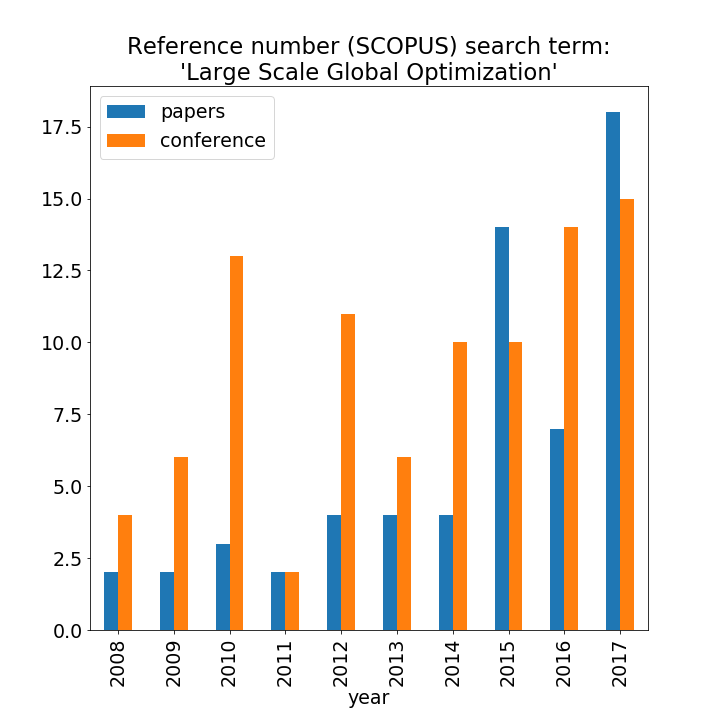
\includegraphics[scale=0.5]{imagenes/LSGO-Evolution}
	\caption{Evolución de las referencias de propuestas de algoritmos LSGO. Fuente: \cite{WCCI-SHADEILS}}
	\label{fig:LSGO-Evolution}
\end{figure}

\subsection{Estado del arte: SOCO 2011 Special Issue}
La \textit{SOCO 2011 Special Issue} cuenta con fuertes propuestas como lo son \textit{A MOS-based dynamic memetic differential evolution algorithm for continuous optimization: a scalability test}\cite{MOS2010}, o MOS-SOCO2011, un algoritmo que basándose en la utilización del framework MOS (Multiple Offspring Sampling), es capaz de \textbf{combinar distintas estrategias de búsqueda} sin tener ninguna fuga; se combinan en este caso un algoritmo de \textbf{evolución diferencial (DE)} y la primera de las tres búsquedas locales del algoritmo MTS\cite{MTS-LSGO}, la \textbf{MTS-LS1}.

Ajustando la participación de cada técnica en base a una función de participación híbrida que favorece la utilización de aquella técnica que ha desempeñado mejor en base a dos medidas distintas, el algoritmo es capaz de obtener resultados muy competitivos, logrando vencer a los demás contrincantes en la competición.
 
Teniendo en cuenta que la evolución diferencial (DE)\cite{DE} es considerada actualmente una de las técnicas más potentes en cuanto a optimización continua, otra propuesta interesante a tener en cuenta de esta misma competición es \textit{Scalability of generalized adaptive differential evolution for large-scale continuous optimization (GaDE)}\cite{GaDE}, una generalización del DE adaptativo en el que a través de una distribución de probabilidad es capaz de \textbf{estimar el valor de cada uno de los parámetros para cada individuo} de la población. Esto se consigue haciendo que la distribución de probabilidad oscile en cada generación en función de las mejoras en fitness de cada individuo, lo que le confiere una gran potencia al algoritmo y se situa como fuerte candidato a solución.

\subsection{Estado del arte: SOCO 2013}

Aunque las propuestas del CEC 2012 no llamen significativamente la atención, por tratarse de técnicas parecidas a las del SOCO 2011 pero con ligeros cambios, en las del \textbf{CEC 2013} se encuentran candidatos muy interesantes como lo son el \textit{Large Scale Global Optimization: experimental results with MOS-based hybrid algorithms}\cite{MOS2013}, técnica que combina un algoritmo genético con dos búsquedas locales muy conocidas y potentes, otra vez, a través del framework MOS: la del algoritmo \textbf{Solis Wets}\cite{SolisWets} y la \textbf{MTS-LS1 Reduced}, una modificación de la MTS-LS1\cite{MTS-LSGO} desarrollada exclusivamente para esta competición donde son optimizadas aquellas variables que contribuyen en mayor medida a una mejora en la calidad de las soluciones.

En esta misma sesión disponemos de una entrada que llama la atención en particular. A pesar de quedar en tercer lugar dentro de esta competición, \textit{Scaling up Covariance Matrix Adaptation Evolution Strategy using cooperative coevolution}\cite{CC-CMAES} o (CC-CMA-ES) es interesante debido a la formulación de la propuesta: dividir el problema en subproblemas más pequeños que serán optimizados utilizando la técnica evolutiva de adaptación por matrices de covarianza CMA-ES. Considerando la dimensionalidad del problema presentado en este trabajo, estrategias de descomposición o subdivisión en problemas más pequeños se postulan como plausibles alternativas a tener en cuenta de cara al estudio.

\subsection{Estado del arte: WCCI 2018 Competition on LSGO}

Finalmente, observando los resultados de la más reciente competición en materia de LSGO,la \textbf{Special Session and Competition on Large-Scale Global Optimization, WCCI 2018} se proponen dos algoritmos que, dada las características y los resultados que obtienen, llaman la atención de manera significativa. Los artículos referentes a ambas propuestas, \textit{SHADE with Iterative Local Search for Large-Scale Global Optimization}\cite{SHADEILS} y \textit{LSHADE-SPA Memetic Framework for Solving Large Scale Problems}\cite{ML-SHADE-SPA}, se encuentran actualmente bajo publicación, pero los resultados y toda la información referente a estos se encuentra disponible.

El primero, SHADEILS, es un algoritmo con una construcción muy similar a una propuesta anterior denominada IHDELS\cite{IHDELS} pero con tres principales diferencias que lo sitúan por encima de su antecesor: mecanismo de \textbf{elección de LS mejorada}, mecanismo de \textbf{reinicio de la población} y el uso de \textbf{SHADE}\cite{SHADE} en vez de SaDE. 

Se elige una LS de entre  MTS-LS1\cite{MTS-LSGO} y L-BFGS-S\cite{LBFGSB}, siendo ambas complementarias: mientras que la primera es rápida pero sensible a rotaciones del sistema de coordenadas, la segunda es mas lenta pero insensible a este tipo de rotaciones. Además, al utilizar SHADE, autoajusta sus parámetros basado en la \textit{historia} y manteniendo la población entre iteraciones, consigue intensificar el proceso de exploración. 

Por otra parte el segundo, ML-SHADE-SPA, es un framework que utiliza \textbf{tres algoritmos basados en poblaciones} para el proceso de \textbf{exploración} (LSHADE-SPA, EADE y ANDE), mientras que el proceso de \textbf{explotación} es llevado a cabo por una \textbf{versión modificada del algoritmo MTS}. Introduce además la idea de \textbf{divide y vencerás}: se mezclan de forma aleatoria las dimensiones y se resuelven de forma separada. Este proceso es completamente independiente de cualquier tipo de información, esto es, las particiones se realizan sin tener en cuenta ninguna suposición acerca de la estructura del problema, añadiendo robustez al algoritmo y confiriéndole un grado de generalización que le permite hacer frente a disintos problemas siguiendo el mismo enfoque.

Cabe destacar que estos dos algoritmos han logrado desbancar al, hasta este año, algoritmo considerado como estado del arte, el mencionado anteriormente MOS, por lo que son los más fuertes candidatos a tener en cuenta en este estudio. Para finalizar, se revisarán las propuestas de algoritmos de descomposición de variables y las posibles ventajas que puede aportar a favor de la resolución del problema tratado en este trabajo.

\section{Estado del arte: algoritmos de descomposición de variables}
NOTA: QUIZA TAMBIEN SEA NECESARIO EXPLICAR EN QUE SE BASAN LOS BENCHMARKS...


\section{Crítica al estado del arte}

Tras analizar los puntos fuertes de las actuales técnicas de resolución de problemas en el ámbito de Big Optimization, el siguiente punto a revisar tiene que ver con la \textbf{identificación de las principales deficiencias} de las técnicas a nivel estructural y de eficiencia y eficacia, con el objetivo de justificar el desarrollo de este trabajo.

El primer punto a considerar es la \textbf{elevada complejidad estructural} de muchas de las técnicas propuestas: a pesar de responder de forma satisfactoria a los benchmarks, su estructura interna muchas veces añade complejidad al problema, ya sea por disponer de \textbf{técnicas de exploración o explotación costosas} a nivel computacional o por perjudicar el \textbf{balance exploración-explotación}, lo que finalmente repercute en la calidad de las soluciones. Técnicas como las basadas en el framework MOS o las de optimización multiobjetivo son sumamente complejas a nivel tanto conceptual como estructural.

La siguiente cuestión esta directamente relacionada con la anterior y es el \textbf{excesivo coste computacional en tiempo} que es necesario para obtener una solución relativamente sensata para este tipo de problemas. No es especialmente preocupante con dimensiones de, por ejemplo, 1000 variables, pero para el problema del EEG donde se manejan hasta 4864 variables se hace completamente inviable el proponer una solución para un problema médico del mundo real. 

Con la formulación uniobjetivo, donde se \textbf{minimiza} a la vez la \textbf{pérdida de información} y la \textbf{prevalecencia de artifacts} tras el proceso de limpieza del EEG, algoritmos como MAGA tardan alrededor de dos horas para el problema sin ruido, siendo el tiempo casi una hora superior cuando se trata de problemas con ruido. Para la formulación multiobjetivo, la representación frente al dominio del tiempo no es siquiera planteada con algoritmos como MOEA/D o NSGA-II, que a pesar de proveer soluciones razonables, siguen empleando demasiado tiempo de computación.

Estos dos preceptos reafirman la \textbf{imposibilidad} de tratar el problema con este tipo de algoritmos, por lo que son necesarias técnicas no más potentes pero si \textbf{más rápidas y con menor sensibilidad al ruido}. De otra forma, una técnica propuesta no tendrá utilidad real futura si se busca aplicarla a un ámbito de tiempo real, como se comentaba en el anterior capítulo, lo que repercutiría de forma negativa en el intento de mejora de la calidad de vida de muchas personas.

Por último mencionar que la gran mayoria de los algoritmos propuestos, sino todos, han seguido una \textbf{lenta evolución} en cuanto a publicaciones efectivas tal y como se puede ver en la figura \ref{fig:LSGO-Evolution}; aquí se representa el hecho de que, hasta hace apenas tres años, la gran mayoría de propuestas se remitían únicamente a los congresos, conferencias y competiciones, siendo estudiadas y evaluadas sobre benchmarks poco representativos del panorama del LSGO actual. En resumen, sin \textbf{propuestas lo suficientemente potentes} como para hacer frente a problemas de optimización del mundo real como lo es en este caso el del EEG.

\section{Propuesta}\label{Propuesta}

El estado del arte actual abre una posibilidad de estudio sobre un problema real de cara a paliar los inconvenientes reflejados anteriormente, tomando como punto de referencia el problema del EEG. El estudio se centrará principalmente en llevar a cabo una \textbf{adaptación híbrida de los algoritmos} considerados \textit{state-of-the-art} de forma que sean capaces de procesar la función objetivo que representa el problema del EEG y ser capaz de proveer resultados que solucionarán, en caso tal, las deficiencias anteriormente expuestas.

Mediante un estudio experimental lo suficientemente completo, se pretende dar respuesta y una posibile solución a los tres inconvenientes destacados en el apartado anterior. Encontrar técnicas potentes en las que \textbf{prime una calidad de soluciones alta}, mejor o igual a la propuesta por el algoritmo \textbf{MAGA} (dado el enfoque uniobjetivo elegido), que será el algoritmo de referencia con el que comparar. 

Esta técnica también ha de dar solución a los dos primeros problemas: la \textbf{complejidad conceptual-estructural debe ser la mínima posible} y los \textbf{tiempos de respuesta efectivos deben ser razonablemente adecuados} a la naturaleza del problema cuando se aplica a un entorno de tiempo real. De esta forma, aunque un algoritmo sea considerado estado del arte en la actual literatura, no se tendría en consideración alguna de cara a la resolución de un problema de optimización real de miles de variables, siendo únicamente válido en términos de evaluaciones frente a benchmarks.

Aquel algoritmo que muestre el desempeño más adecuado de acuerdo a las anteriores primitivas, independientemente de si ha conseguido solventar de forma total los tres escenarios anteriores, se someterá a estudio bajo un \textbf{algoritmo de descomposición de variables}, para comprobar si la \textbf{optimización por separado de grupos de variables} implica realmente una \textbf{reducción de la dimensionalidad} a nivel individual del problema y emitir un juicio en cuanto a si se consigue mejorar los resultados que proporciona el algoritmo base elegido. En caso favorable, se propondrá una solución lo suficientemente respaldada de cara a ser implementada en sistemas BCIs donde se pueda estudiar de forma mucho mas eficiente y efectiva un EEG cuantitativo, incluso en entornos donde se requiera respuesta en tiempo real.